%! Author = zhiweizhang
%! Date = 10.06.25

\chapter{Methodology}\label{chapter:methodology}

In this section, we will discuss our training data first, then we
discuss about data preprocessing steps, at the end we talk about the
algorithms we used.

\section{Data Collection}
\label{sec:data-collection}

To develop a robust image classifier capable of distinguishing Nazi symbols from other visual elements, a
comprehensive dataset containing both positive and negative image classes was constructed. The datasets were sourced
from two major platforms:

\begin{itemize}
  \item \textbf{Roboflow}: Provided labeled datasets containing Nazi symbols such as swastikas, SS bolts, and the
  Black Sun. These datasets constituted the positive class and were selected based on symbol relevance, label
  accuracy, and visual diversity.

  \item \textbf{Kaggle}: Offered general-purpose datasets comprising everyday objects, street scenes, and
  non-extremist logos. These images formed the negative class, helping the model learn to discriminate between Nazi
  iconography and unrelated content, thereby minimizing false positives.
\end{itemize}

The collected datasets varied in resolution, label format, class granularity, and symbolic diversity. A summary
table including dataset names, descriptions, and sources is provided in Table~\autoref{tab:dataset_summary}.

All datasets were obtained under open-use or research-friendly licenses, in compliance with the terms specified by
their respective platforms and contributors. To ensure data integrity and ethical compliance, the following steps
were taken:

\begin{itemize}
  \item Manual inspection was performed on each dataset to verify label accuracy and image quality.
  \item Nazi symbol datasets were annotated and filtered into predefined classes based on visual traits and
  historical context, guided by taxonomies from the Anti-Defamation League (ADL) and academic research on hate iconography.
  \item Duplicate or near-duplicate images across datasets were removed to prevent data leakage.
\end{itemize}

The aggregated dataset was randomly partitioned into three subsets: 70\% for training, 15\% for validation, and 15\%
for testing. Care was taken to avoid overlap of symbol instances across these partitions.

\begin{table}[htbp]
\centering
\small
%\renewcommand{\arraystretch}{2}
\resizebox{\textwidth}{!}{
\begin{tabular}{clcl}
\toprule
\textbf{Platform} & \textbf{Dataset Name / Description} & \textbf{Purpose} & \textbf{Notes} \\
\midrule
Roboflow & detect Dataset~\parencite{detect-lhuia_dataset} & Positive Class & Swastika and related Nazi symbols \\

Roboflow & swastika Dataset (imgann)~\parencite{swastika-o7bde_dataset} & Positive Class & Swastika symbol detection \\

Roboflow & swastika Dataset (Darja Nechaeva)~\parencite{swastika-uw8xt_dataset} & Positive Class & Historical swastika variations \\

Roboflow & swastika\_detect Dataset~\parencite{swastika_detect_dataset} & Positive Class & Swastika detection for moderation \\

Roboflow & symbols Dataset~\parencite{symbols-w93jw_dataset} & Positive Class & Includes general and hate symbols \\

Roboflow & violent object Dataset~\parencite{violent-object_dataset} & Positive Class & Hate symbols and violent imagery \\

Roboflow & Swastiki\_Net Dataset~\parencite{swastiki_net_dataset} & Positive Class & Swastika symbol classification \\

Roboflow & Content Moderation Dataset~\parencite{content-moderation-fwj5b_dataset} & Positive Class & Multiple harmful or extremist symbols \\

Roboflow & Swastika\_Detection Dataset~\parencite{swastika_detection_dataset} & Positive Class & Swastikas in different contexts \\

Kaggle & 100 Sports Image Classification~\parencite{100_sport_image_classification_dataset} & Negative Class & Neutral sports images \\

Kaggle & Car vs Bike Classification Dataset~\parencite{car_bike_classification_dataset} & Negative Class & Background class diversity \\

Kaggle & People Clothing Segmentation~\parencite{people_clothing_segmentation_dataset} & Negative Class & Background objects, neutral content \\

Kaggle & Fruits and Vegetables Dataset~\parencite{fruit_and_vegetable_image_recognition_dataset} & Negative Class & For reducing false positives \\

Kaggle & Animal Image Dataset~\parencite{animal_image_dataset} & Negative Class & Animal images for neutral comparison \\

Kaggle & Kids and Adults Detection~\parencite{kids_and_adults_detection_dataset} & Negative Class & Human figures, non-extremist \\

Kaggle & SCOOBY DOO Classification~\parencite{scooby_doo_classification_dataset} & Negative Class & Cartoon data for variance \\

Kaggle & Low Light Animals~\parencite{subrata_sarkar_2025} & Negative Class & Low-light conditions for robustness \\

Kaggle & AI vs Human-Generated Images~\parencite{ai_vs_human_generated_images_dataset} & Negative Class & Diverse image source simulation \\
\bottomrule
\end{tabular}
}
\caption{Summary of datasets used in this thesis for training, validation, and testing.}
\label{tab:dataset_summary}
\end{table}

\subsection{Nazi Symbol Taxonomy and Distribution}

The final dataset includes \textbf{22 distinct Nazi-related symbols}, ranging from widely recognized emblems (e.g.,
swastika, SS bolts) to lesser-known variants (e.g., Wolfsangel, Kolovrat). These were selected based on their
documented use in historical Nazi insignia, far-right propaganda, and contemporary neo-Nazi subcultures. A visual
overview of representative images is shown in Figure~\ref{figure:nazi-symbol-examples}, while
Section~\autoref{section:symbol-description} provides full symbol descriptions.

\begin{figure}[ht]
  \centering
  
\includegraphics[scale=0.55]{nazi-symbol-examples}
  \caption{Example images from 22 Nazi symbol classes.}
  \label{figure:nazi-symbol-examples}
\end{figure}

\section{Nazi Symbol Description}
  \label{section:symbol-description}

The Nazi symbols are mainly from Roboflow with labels. The symbols are defined as follows:

\begin{itemize}
  \item \textbf{Sonnenrad}: The sonnenrad, or sunwheel, is an ancient symbol
  from Norse and Celtic cultures that was appropriated by the Nazis to
  promote an idealized "Aryan" heritage. Its many variations include forms
  of the swastika and Celtic Cross, and it was used by the Nazi Party,
  SA, and SS. Today, it is commonly used by neo-Nazis and white
  supremacists, especially a version with two concentric circles and
  crooked rays, sometimes featuring a swastika in the center.
  \item \textbf{Flash and circle}: The Flash and Circle is a symbol featuring
  a lightning bolt within a circle, originally used by the British Union
  of Fascists in the 1930s. It was meant to represent action within unity
  and has since been adopted by neo-fascist and white supremacist groups.
  Though less common today, it remains a recognizable hate symbol associated
  with fascist ideology.
  \item \textbf{Broken Sun Cross}: Symbols featuring an equilateral cross enclosed
  in a circle have appeared in various cultures since the Bronze Age. Since
  the 1930s, a version with ‘broken’ arms resembling a swastika gained far-right
  associations. It was used by the German Faith Movement and later as insignia
  for two Waffen SS divisions.
  \item \textbf{The Happy Merchant}: The Happy Merchant is an antisemitic meme
  depicting a Jewish man with exaggerated, stereotypical features, often used
  by white supremacists to promote hate. It originated from racist artwork
  by cartoonist Nick Bougas, who used the pseudonym “A. Wyatt Mann.” His
  offensive cartoons, widely circulated in the 1980s and 1990s, were often
  published by white supremacist Tom Metzger.
  \item \textbf{Hitler}: The images of Adolf Hilter.
  \item \textbf{Nazi salute}: The Nazi salute, also known as the Hitler salute
  or Sieg Heil salute, was a gesture used
  in Nazi Germany to show loyalty to Adolf Hitler and the Nazi Party, typically
  accompanied by phrases like "Heil Hitler" or "Sieg Heil". Inspired by the
  Italian Fascist salute, it became an official Nazi greeting in 1926 and
  was mandatory for civilians but optional for military personnel until
  1944. Today, the salute is banned in several countries—including Germany,
  Austria, and Slovakia—and is considered hate speech or a criminal act in
  many others if used to promote Nazi ideology.
%  \item \textbf{Neo-Nazi emblems}: Neo-Nazi emblems are symbols used by modern
%    white supremacist and neo-Nazi groups to express their extremist beliefs
%    and allegiance to Nazi ideology. These emblems often include modified or
%    obscure versions of historical Nazi symbols, such as the swastika, sonnenrad,
%    or runes, to avoid legal restrictions or public scrutiny. While some are
%    direct revivals, others are new creations that serve the same purpose of
%    spreading hate and promoting white nationalist ideas. In this study, it includes
%    symbols from various far-right extremist groups, such as Atomwaffen Division emblem,
%    Blood \& Honor emblem, Celtic Cross, Combat 18 emblem, Golden Dawn, Hammerskins emblem,
%    Identitarian movement emblem, Kolovrat, National Rebirth of Poland emblem,
%    Popular front emblem. Since only a limited number of images were available for
%    each group, they were consolidated under a single "Neo-Nazi" class for classification purposes.
  \item \textbf{Yellow badge}: The Yellow badge was a cloth patch, usually in
  the shape of a Star of David, that Jews were forced to wear by the Nazis
  to identify and segregate them. It symbolized persecution and was used to
  mark Jews publicly, contributing to their dehumanization and eventual
  deportation. Today, it stands as a powerful symbol of the Holocaust and
  the oppression of Jewish people.
  \item \textbf{Siegrune}: The Siegrune, or "S rune", is a lightning-bolt-shaped
  symbol used by the Nazi SS to represent victory ("Sieg" in German). It was
  adapted from ancient runic alphabets and became one of the most recognizable
  symbols of the SS, often displayed as a double rune on uniforms and insignia.
  Today, it is widely recognized as a hate symbol and is banned or restricted
  in several countries due to its association with Nazi ideology.
  \item \textbf{SS Skull}: The SS skull, also known as the "Totenkopf" ("death's head"),
  was a symbol used by the Nazi SS to represent loyalty unto death and intimidation.
  It was prominently featured on SS uniforms, especially those of the elite units
  and concentration camp guards. Today, it is considered a hate symbol due to
  its strong association with the crimes and ideology of the SS and the Nazi regime.
  \item \textbf{Sturmabteilung emblem}: The Sturmabteilung (SA) emblem was the
  symbol of the Nazi Party's paramilitary wing, known for its violent tactics
  and support for Adolf Hitler's rise to power. The emblem typically featured
  a stylized version of the SA initials, often accompanied by a swastika.
  It represented the SA's role in enforcing Nazi ideology and intimidation,
  and the emblem is now recognized as a symbol of hate and fascism.
  \item \textbf{Swastika}: The Swastika is an ancient symbol, originally used in
  various cultures to represent good luck, prosperity, and well-being. However,
  it was appropriated by the Nazi Party in the 1920s, becoming a powerful
  symbol of their ideology and representing white supremacy, hate, and
  anti-Semitism. Today, it is widely recognized as a symbol of Nazi oppression
  and is illegal in many countries due to its association with hate and violence.
  \item \textbf{Wolfsangel}: The Wolfsangel is a symbol originally used in medieval
  Europe, representing a wolf trap, and later adopted by Nazi and neo-Nazi
  groups. It was used by Nazi units during World War II, including the Waffen-SS,
  and has become associated with white supremacy and fascist ideologies. Today,
  the Wolfsangel is a recognized hate symbol, often used by extremist groups
  to promote Nazi beliefs.
  \item \textbf{Atomwaffen Division emblem}:The Atomwaffen Division emblem is a symbol
  used by a violent neo-Nazi terrorist group known for promoting accelerationism and
  engaging in acts of domestic terrorism. The emblem typically features a stylized
  radiation warning symbol, representing the group's fascination with chaos,
  destruction, and nuclear war. It is widely recognized as a hate symbol and is
  associated with extremist violence, white supremacy, and far-right terrorism.
  \item \textbf{Blood \& Honor emblem}: The Blood \& Honour emblem represents an international
  neo-Nazi network that promotes white supremacist music and ideology. The name comes
  from the Hitler Youth motto "Blut und Ehre" (Blood and Honor), and the emblem often
  includes those words along with fascist symbols like runes or laurel wreaths. It
  is widely recognized as a hate symbol linked to racist propaganda, violence,
  and far-right extremism.
  \item \textbf{Celtic Cross}: The Celtic Cross is an ancient symbol with religious
  and cultural origins in Celtic Christianity, featuring a cross with a circle
  around the intersection. While it remains a legitimate cultural and religious
  symbol, white supremacists have adopted a simplified version as a symbol of white
  identity and nationalism. This version is now widely recognized as a hate symbol
  in extremist contexts.
  \item \textbf{Combat 18 emblem}: Combat 18 is a violent neo-Nazi organization, with the
  number "18" representing the initials A and H (Adolf Hitler). Its emblem typically
  includes the number or stylized letters alongside other far-right imagery. The group
  is known for promoting white supremacy and terrorism, and its emblem is a symbol of
  hate and violence.
  \item \textbf{Golden Dawn}: Golden Dawn is a far-right political party from Greece known for its neo-Nazi ideology
  and involvement in violent, xenophobic acts. Its emblem resembles a Greek meander pattern, often compared to a
  swastika due to its stylized, angular design. Though once politically active, the group has been widely condemned
  and legally prosecuted for its extremist activities.
  \item \textbf{Hammerskins emblem}: The Hammerskins emblem features two crossed hammers, symbolizing the group's
  slogan "Hammerskins Nation" and white power. This violent white supremacist group is rooted in the skinhead
  movement and is heavily involved in hate music and racist activism. The emblem is a well-known hate symbol tied to
  global neo-Nazi networks.
  \item \textbf{Identitarian movement emblem}: The Identitarian Movement emblem typically features a yellow circle
  with a black Greek lambda symbol, inspired by the Spartan shield. This far-right European movement promotes
  anti-immigration and ethnonationalist ideologies under the guise of cultural preservation. Although presented with
  modern, clean branding, the emblem is associated with white nationalist beliefs.
  \item \textbf{Kolovrat}: The Kolovrat is an ancient Slavic symbol representing the sun and cosmic cycles, used
  historically in pagan contexts. In recent years, it has been appropriated by Slavic neo-Nazis and white
  supremacists as a symbol of ethnic purity and nationalist pride. While some use it in a cultural or historical
  sense, its association with extremist ideology marks it as a hate symbol in certain contexts.
  \item \textbf{National Rebirth of Poland emblem}: The National Rebirth of Poland (NOP) emblem represents a
  far-right nationalist party in Poland known for its anti-Semitic and xenophobic views. The emblem often
  incorporates stylized nationalist imagery, including swords or eagles, designed to evoke Polish strength and
  purity. It is associated with extremist rhetoric and far-right political activism in Poland.
  \item \textbf{Popular front emblem}: The Popular Front emblem is used by a range of nationalist or fascist groups,
  often combining traditional nationalist symbols like eagles or stars with militaristic imagery. Though the term "
  Popular Front" historically referred to leftist coalitions, in extremist contexts, it can represent
  ultra-nationalist, anti-democratic movements. The emblem typically signals far-right or authoritarian ideologies.
%  \item \textbf{Doppelsiegrune}: The Doppelsiegrune, or "double Siegrune," features two lightning-bolt-like runes
%  and was the official insignia of the Nazi SS. It symbolized power, obedience, and loyalty to Adolf Hitler and
%  became one of the most infamous emblems of the Nazi regime. Today, it is banned or heavily restricted in many
%  countries and is recognized worldwide as a symbol of hate and terror.
\end{itemize}

\subsection{Dataset Structuring for Tasks}

To accommodate the differing objectives of the binary and multi-class classification tasks, the dataset was
structured as follows:

\begin{itemize}
    \item \textbf{Binary Classification (Symbol Detection):}
    All images containing any of the 22 Nazi-related symbol classes were merged into a single positive class labeled
    \item \textit{Nazi}. Images without Nazi-related content were labeled as \textit{non-Nazi}.
    The resulting dataset consisted of approximately \textbf{2,300 Nazi images} and \textbf{99,000 non-Nazi images},
    reflecting a 1:42 class ratio. This structuring supports a general detection task, identifying whether any Nazi
    symbol is present in an image.

    \item \textbf{Multi-Class Classification (Symbol Identification):}
    This task focused exclusively on the 22 Nazi symbol categories. Only images labeled with a Nazi symbol were
    included, preserving their individual class labels.
    The dataset for this task included a total of approximately \textbf{2,300 images}, with class sizes ranging from
    tens to hundreds of examples per symbol. Due to this variability, the dataset exhibited significant class
    imbalance, which posed challenges for model generalization across all symbol categories.
\end{itemize}

This structuring strategy ensured that the dataset aligned with the goals of each classification task: broad
detection capability in the binary case and fine-grained categorization in the multi-class case.


Due to the limited number of images in several classes, a new category labeled \textit{Neo-Nazi} was created to
group together symbol classes with very few examples. This regrouping allows the classifier to generalize better and
prevents overfitting on sparsely represented classes. Table~\autoref{tab:symbol-distribution} presents the distribution
of images in both the main Nazi-related symbol classes and the individual symbol types grouped under the
\textit{Neo-Nazi} label. The regrouping also improves class balance in the multi-class classification task, while
retaining interpretability for downstream applications.

%! Author = zhiweizhang
%! Date = 10.06.25

% Preamble
\begin{table}[ht]
  \begin{subtable}[c]{0.5\textwidth}
    \centering
    \begin{tabular}{|l|c|}
      \hline
      \textbf{Class} & \textbf{Images} \\
      \hline\hline
      Sonnenrad & 152 \\\hline
      Flash and circle & 13 \\\hline
      Broken Sun Cross & 21 \\\hline
      The Happy Merchant & 39 \\\hline
      Hitler & 228 \\\hline
      Nazi salute & 6 \\\hline
      Neo-Nazi & 188 \\\hline
      Yellow badge & 4 \\\hline
      Siegrune & 311 \\\hline
      SS Skull & 257 \\\hline
      Sturmabteilung emblem & 11 \\\hline
      Swastika & 1070 \\\hline
      Wolfsangel & 38 \\\hline
    \end{tabular}
    \subcaption{Regrouped symbol distribution}
  \end{subtable}
\hfill
  \begin{subtable}[c]{0.5\textwidth}
    \centering
    \begin{tabular}{|l|c|}
      \hline
      \textbf{Class} & \textbf{Images} \\
      \hline\hline
      Atomwaffen Division & 8 \\\hline
      Blood \& Honor emblem & 25 \\\hline
      Celtic Cross & 51 \\\hline
      Combat 18 emblem & 6 \\\hline
      Golden Dawn & 19 \\\hline
      Hammerskins emblem & 12 \\\hline
      Identitarian movement & 11 \\\hline
      Kolovrat & 38 \\\hline
      National Rebirth of Poland & 10 \\\hline
      Popular Front emblem & 8 \\\hline
    \end{tabular}
    \subcaption{Neo-Nazi Symbol distribution}
  \end{subtable}

  \caption{Symbol distribution}
  \label{tab:symbol-distribution}
\end{table}

\subsection{Sample Images}

Figure~\autoref{fig:dataset-samples} presents representative examples from both classes, illustrating the visual
diversity and annotation consistency.

\begin{figure*}[ht]
  \centering
  \begin{subfigure}[t]{0.48\textwidth}
    \centering
    
\includegraphics[scale=0.37]{nazi-examples}
    \caption{Sample images containing Nazi symbols}
  \end{subfigure}%
  \hfill
  \begin{subfigure}[t]{0.48\textwidth}
    \centering
    
\includegraphics[scale=0.39]{non-nazi-examples}
    \caption{Sample images not containing Nazi symbols}
  \end{subfigure}
  \caption{Examples from the positive and negative classes}
  \label{fig:dataset-samples}
\end{figure*}

\noindent
All data collection procedures were conducted in accordance with academic ethical standards. No personal or
sensitive identifiable content was included, and all datasets were used strictly for research purposes aimed at
countering extremism.

\section{Algorithms}
To evaluate the effectiveness of different machine learning approaches in Nazi symbol detection and classification,
we experimented with a diverse set of models. These include both modern deep learning architectures and traditional
machine learning algorithms, allowing us to compare performance across various paradigms and computational complexities.

\subsection{YOLO (You Only Look Once)}
YOLO is a real-time object detection framework that treats detection as a single regression problem, directly
predicting bounding boxes and class probabilities from full images. YOLO processes the entire image in one forward
pass, offering a trade-off between speed and accuracy that is well-suited for applications requiring real-time
inference. While primarily intended for detection tasks, YOLO can be adapted for classification by interpreting the
most confident detection as the image label. In this study, we adopt YOLOv11 for its enhanced speed and robustness,
leveraging its latest improvements in backbone design and label assignment.

\subsection{ResNet (Residual Network)}
ResNet is a convolutional neural network that employs residual learning to ease the training of very deep networks
by introducing identity shortcut connections. This design mitigates the vanishing gradient problem, enabling
efficient training of architectures with hundreds of layers. ResNet has demonstrated strong performance in image
classification benchmarks. We utilize ResNet-50, a 50-layer deep variant, for its proven balance between model
complexity and classification accuracy.

\subsection{EfficientNet}
EfficientNet is a family of CNN architectures that systematically scales depth, width, and resolution using a
compound coefficient, resulting in a series of models that achieve state-of-the-art accuracy with significantly
fewer parameters. EfficientNet is highly efficient in resource usage, making it suitable for large-scale image
classification on limited hardware. In our experiments, it serves as a lightweight alternative to deeper networks
without substantial sacrifice in accuracy.

\subsection{Vision Transformer (ViT)}
The Vision Transformer adapts the transformer architecture from NLP to vision tasks by dividing images into patches
and processing them as a sequence of tokens. It eliminates convolutions entirely and instead relies on
self-attention mechanisms to capture long-range dependencies and global context. ViT has shown competitive or
superior performance compared to CNNs when trained on sufficiently large datasets. We include ViT in our comparison
to evaluate the effectiveness of transformer-based models in classifying visual symbols with complex semantics.

\subsubsection{OpenCLIP}
OpenCLIP is an open-source implementation of CLIP (Contrastive Language–Image Pretraining), a vision-language model
trained on a large-scale dataset of image-text pairs. OpenCLIP learns a shared embedding space for both modalities,
allowing for zero-shot classification by comparing image embeddings to text prompt embeddings. We use OpenCLIP both
in zero-shot mode and as a feature extractor, offering a flexible and semantically rich representation of images
aligned with natural language descriptions.

\subsection{Moondream}
Moondream is a compact multimodal model optimized for low-resource vision-language tasks. Though not explicitly
designed for image classification, it can be adapted for lightweight classification through the use of prompt-based
text-image comparisons. Its strength lies in efficient on-device performance, making it ideal for scenarios with
constrained computational resources. We explore Moondream as a potential solution for mobile or embedded
classification settings.

\subsubsection{OpenCLIP as Encoder with Classical Machine Learning Classifiers}
To leverage the semantic richness of OpenCLIP’s embeddings, we also employ it as a frozen feature encoder. The
resulting vector representations are then used as input to traditional machine learning classifiers. This two-stage
pipeline allows rapid experimentation with interpretable and computationally efficient models, particularly
advantageous for small datasets or when deep learning is computationally prohibitive. A summary of the key
characteristics of used classification algorithms is provided in Table~\ref{tab:summary-classification-algorithms}.

\paragraph{Classic Classifiers Used:}
\begin{itemize}
  \item \textbf{Logistic Regression:} A linear probabilistic model ideal for binary classification problems.
  \item \textbf{SGD Classifier:} An efficient linear classifier using stochastic gradient descent, scalable to large
  datasets.
  \item \textbf{K-Nearest Neighbors (KNN):} A non-parametric algorithm that assigns labels based on the closest
  training examples in feature space.
  \item \textbf{Support Vector Classifier (SVC):} A margin-based classifier effective for high-dimensional data.
  \item \textbf{Decision Tree Classifier:} A hierarchical model that splits data based on feature thresholds,
  enabling interpretable decision-making.
  \item \textbf{Bagging Classifier:} An ensemble of decision trees trained on bootstrapped samples to reduce variance.
  \item \textbf{AdaBoost Classifier:} A sequential ensemble that emphasizes misclassified samples to improve accuracy.
  \item \textbf{Gradient Boosting Classifier:} Builds strong predictors by optimizing a loss function in a
  stage-wise fashion using weak learners.
  \item \textbf{Random Forest Classifier:} An ensemble of decision trees with random feature selection, offering
  robustness and high accuracy.
  \item \textbf{Voting Classifier:} Combines predictions from multiple base models (e.g., Logistic Regression,
  Random Forest, Linear SVC) via soft or hard voting to improve overall performance.
\end{itemize}

%! Author = zhiweizhang
%! Date = 10.06.25

% Preamble
\begin{table}[ht]
  \centering
  \resizebox{\textwidth}{!}{
    \begin{tabular}{lccccc}
    \toprule
    \textbf{Classifier}          & \textbf{Model Type} & \textbf{Linear}       & \textbf{Ensemble} & \textbf{Interpretable} & \textbf{Scalable} \\
    \midrule
    Logistic Regression          & Parametric          & Yes                   & No                & High                   & High              \\
    SGD Classifier               & Parametric          & Yes                   & No                & Moderate               & Very High         \\
    KNN Classifier               & Instance-based      & No                    & No                & Low                    & Low               \\
    SVC                          & Parametric          & Yes                   & No                & Moderate               & High              \\
    Decision Tree Classifier     & Non-parametric      & No                    & No                & High                   & Moderate          \\
    Bagging Classifier           & Non-parametric      & No                    & Yes               & Moderate               & High              \\
    AdaBoost Classifier          & Non-parametric      & No                    & Yes               & Low to Moderate        & Moderate          \\
    Gradient Boosting Classifier & Non-parametric      & No                    & Yes               & Low                    & Moderate          \\
    Random Forest Classifier     & Non-parametric      & No                    & Yes               & Moderate               & High              \\
    Voting Classifier            & Hybrid              & Depends on estimators & Yes               & Low                    & High              \\
    \bottomrule
    \end{tabular}
  }
  \caption{Summary of classification algorithms and their key characteristics}
  \label{tab:summary-classification-algorithms}
\end{table}

\section{Data Preprocessing}

To ensure the robustness and consistency of our models, we applied a comprehensive data preprocessing pipeline that
includes resizing, normalization, and offline data augmentation. These steps are essential for reducing noise,
simulating real-world variations, and enabling efficient training.

\begin{itemize}
  \item \textbf{Resizing}: All images were resized to a fixed resolution to ensure uniform dimensions across the
  dataset. This not only standardizes input for model compatibility but also improves computational efficiency
  during both training and inference.

  \item \textbf{Normalization}: Each image was normalized by scaling pixel values to the range $[0, 1]$ on a per-image
  basis. This helps stabilize the training process and accelerates convergence by ensuring consistent data scaling.

  \item \textbf{Data Augmentation}: We performed offline data augmentation to artificially increase the diversity of
  the training set and enhance model generalization. The augmentations were applied probabilistically to each image
  to simulate realistic variations in appearance. The augmentation techniques included:
  \begin{itemize}
    \item \textit{Conversion to grayscale} to remove color-related variance
    \item \textit{Automatic contrast adjustment} to normalize dynamic range
    \item \textit{Random horizontal and vertical flipping} (50\% probability) to simulate real-world image
    orientation variations
    \item \textit{Random rotation} (±15°) to introduce viewpoint variability
    \item \textit{Random shearing} (vertically ±10° and horizontally ±10°) to simulate perspective distortion
    \item \textit{Random changes in hue, saturation, and brightness} (hue: ±15°, saturation: ±63, brightness: ±38) to
    increase robustness to lighting and color shifts.
    \item \textit{Random exposure changes} to simulate overexposure or underexposure conditions
    \item \textit{Random Gaussian blur} to introduce realistic image imperfections
    \item \textit{Random noise addition} (0.1\% probability) to increase robustness against sensor noise or image
    degradation
  \end{itemize}
  These transformations were chosen to mimic common distortions found in real-world imagery, such as poor lighting,
  camera movement, compression artifacts, and historical degradation, which are especially relevant in the context
  of Nazi symbol detection.

\end{itemize}

All preprocessing steps were implemented using a combination of \texttt{Pillow} and \texttt{OpenCV} in an offline
processing stage. The pipeline was designed to first resize the images, followed by augmentation and normalization.
This ordering ensures computational efficiency and consistency across all samples.

Examples of these preprocessing steps—including augmentation, resizing, and normalization—are illustrated in Figure~\ref{fig:example-preprocessing-steps}.

\begin{figure}[ht]
\begin{subfigure}{.5\textwidth}
  \centering
  
\includegraphics[width=.8\linewidth]{original-example}
  \caption{Original image example.}
\end{subfigure}%
\begin{subfigure}{.5\textwidth}
  \centering
  
\includegraphics[width=.8\linewidth]{augmented-example}
  \caption{Augmented image example.}
\end{subfigure}
\begin{subfigure}{.5\textwidth}
  \centering
  
\includegraphics[width=.53\linewidth]{resized-example}
  \caption{Resized image example.}
\end{subfigure}%
\begin{subfigure}{.5\textwidth}
  \centering
  
\includegraphics[width=.8\linewidth]{normalized-example}
  \caption{Normalized image example.}
\end{subfigure}
\caption{Examples of data preprocessing steps.}
\label{fig:example-preprocessing-steps}
\end{figure}

\section{Model Training}

Each model in this study was trained using specific hyperparameter configurations suited to its architecture and classification task. For all deep learning models, early stopping was applied based on validation loss with a patience of 10 epochs to prevent overfitting. The best-performing model on the validation set was preserved for final evaluation. A summary of the key training hyperparameters is provided in Table~\ref{tab:training-hyperparameters}.

\textbf{ResNet50} was trained for 100 epochs with a batch size of 16 and input image size of $224 \times 224$. Binary cross-entropy (BCE) loss was used for binary classification tasks and categorical cross-entropy (CCE) for multi-class classification. The Adam optimizer was employed with an initial learning rate of $1 \times 10^{-3}$, along with weight decay of $1 \times 10^{-5}$. A 1-cycle learning rate scheduler was used to adjust the learning rate dynamically over the epochs.

\textbf{EfficientNet} was trained for 100 epochs using a batch size of 16 and input size of $224 \times 224$. For binary classification, the Nesterov momentum variant of Adam (NAdam) was used with a learning rate of $2 \times 10^{-3}$, zero weight decay, and a momentum decay of 0.004. For multi-class classification, the Adam optimizer with an initial learning rate of $1 \times 10^{-3}$ was used. In both cases, the model’s fully connected layer was modified to a linear layer, where the number of output features matched the number of classes.

\textbf{Vision Transformer (ViT)} was trained for 100 epochs with a batch size of 16 and input image size of $224 \times 224$. The Adam optimizer with a learning rate of $2 \times 10^{-5}$ was used, and loss functions were selected according to the classification task (BCE for binary, CCE for multi-class).

\textbf{YOLOv11} was trained for 100 epochs with a batch size of 16 and input image size of $224 \times 224$. SGD was used as the optimizer with an initial learning rate of 0.01, momentum of 0.9, and weight decay of 0.0005. Binary cross-entropy and categorical cross-entropy were used for binary and multi-class classification, respectively.

\textbf{OpenCLIP-based models}: When using OpenCLIP as a feature encoder followed by classical machine learning classifiers, embeddings were extracted from resized input images ($224 \times 224$), and classifiers (e.g., logistic regression, SVM, KNN) were trained on these features. These training processes were straightforward and executed on CPU. In contrast, zero-shot classification with OpenCLIP and Moondream did not involve training on the dataset. Instead, classification was performed by measuring the cosine similarity between image and text embeddings, enabling inference without fine-tuning.

All training experiments were conducted on an NVIDIA RTX 4090 GPU with 16 GB VRAM (10 GB available).

%! Author = zhiweizhang
%! Date = 10.06.25

% Preamble
\begin{table}[ht]
\centering
\resizebox{\textwidth}{!}{
\begin{threeparttable}

\begin{tabular}{lcccccc}
\toprule
\textbf{Model}                  & \textbf{Epochs} & \textbf{Batch Size} & \textbf{Input Size} & \textbf{Loss Function} & \textbf{Optimizer} & \textbf{Learning Rate}  \\
\midrule
ResNet-34                       & 100             & 48                  & 224×224             & BCE/CCE\tnote{1}       & Adam               & 1e-3                    \\
EfficientNet-b2 (binary)        & 100             & 48                  & 224×224             & BCE                    & Nadam              & 2e-3                    \\
EfficientNet-b2 (multi)         & 100             & 48                  & 224×224             & CCE                    & Adam               & 1e-3                    \\
ViT                             & 100             & 48                  & 224×224             & BCE/CCE                & Adam               & 2e-5                    \\
YOLOv11                         & 100             & 48                  & 224×224             & BCE/CCE                & SGD                & 0.01                    \\
OpenCLIP + ML                   & –               & –                   & 224×224             & –                      & –                  & –                       \\
Zero-shot (OpenCLIP, Moondream)\tnote{2} & –               & –                   & –                   & –                      & –                  & –                       \\
\bottomrule
\end{tabular}

\smallskip\footnotesize
\begin{tablenotes}
    \item[1] BCE = Binary Cross-Entropy, CCE = Categorical Cross-Entropy.\vfill
    \item[2] Zero-shot models are not trained on the dataset; they use pretrained weights and inference directly.

\end{tablenotes}
\end{threeparttable}
}
\caption{Summary of training hyperparameters used for each model.}
\label{tab:training-hyperparameters}
\end{table}

\begin{figure}[ht]
    \centering
    \begin{tikzpicture}
        \pie[text=legend, radius=3,
            color={blue!60, red!70}] % 99435 + 2338
            {97.7/Non-Nazi, 2.3/Nazi}
    \end{tikzpicture}
    \caption{Pie chart showing binary classification dataset distribution.}
    \label{fig:binary-dataset-pie}
\end{figure}



\begin{figure}[ht]
    \centering
    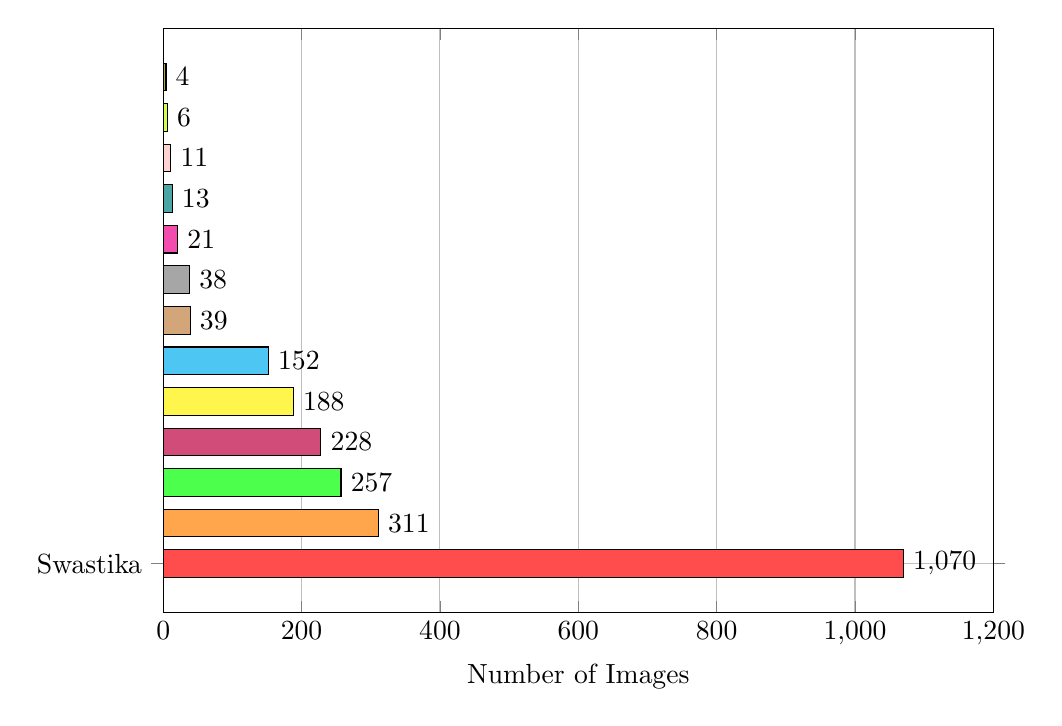
\begin{tikzpicture}
        \begin{axis}[
            xbar,
            bar width=10pt,
            width=\textwidth,
            height=9cm,
            xlabel={Number of Images},
            symbolic y coords={
                swastika,
                siegrune,
                ss\_skull,
                hitler,
                neo-nazi,
                black\_sun,
                happy\_merchant,
                wolfsangel,
                broken\_sun\_cross,
                british\_union\_of\_fascist,
                sturmabteilung\_emblem,
                hitler\_salute,
                judenstern
            },
            ytick=data,
            yticklabels={
                Swastika,
                Siegrune,
                SS Skull,
                Hitler,
                Neo-Nazi,
                Black Sun,
                Happy Merchant,
                Wolfsangel,
                Broken Sun Cross,
                British Union of Fascist,
                Sturmabteilung Emblem,
                Hitler Salute,
                Judenstern
            },
            xmin=0,
            xmax=1200,
            nodes near coords,
            nodes near coords align={horizontal},
            enlarge y limits=0.1,
            grid=major,
            bar shift=0pt,
            ]

            % bars with color coding
            \addplot[fill=red!70] coordinates {(1070,swastika)};
            \addplot[fill=orange!70] coordinates {(311,siegrune)};
            \addplot[fill=green!70] coordinates {(257,ss\_skull)};
            \addplot[fill=purple!70] coordinates {(228,hitler)};
            \addplot[fill=yellow!70] coordinates {(188,neo-nazi)};
            \addplot[fill=cyan!70] coordinates {(152,black\_sun)};
            \addplot[fill=brown!70] coordinates {(39,happy\_merchant)};
            \addplot[fill=gray!70] coordinates {(38,wolfsangel)};
            \addplot[fill=magenta!70] coordinates {(21,broken\_sun\_cross)};
            \addplot[fill=teal!70] coordinates {(13,british\_union\_of\_fascist)};
            \addplot[fill=pink!70] coordinates {(11,sturmabteilung\_emblem)};
            \addplot[fill=lime!70] coordinates {(6,hitler\_salute)};
            \addplot[fill=olive!70] coordinates {(4,judenstern)};
        \end{axis}
    \end{tikzpicture}
    \caption{Dataset distribution of the multi-class classification task.}
    \label{fig:multi-class-dataset-distribution}
\end{figure}
